
\documentclass[letterpaper,hide notes,xcolor={table,svgnames},pdftex,10pt]{beamer}
\def\showexamples{t}

\usecolortheme{crane}
\setbeamertemplate{navigation symbols}{}

\usetheme{MyPittsburgh}
\usepackage{hyperref}
\usepackage{graphicx,xspace}
\usepackage[normalem]{ulem}
\usepackage{multicol}
\usepackage{amsmath,amssymb,amsthm,graphicx,xspace}
\newcommand\SF[1]{$\bigstar$\footnote{SF: #1}}

\usepackage[sfdefault,lf]{carlito}
\usepackage[T1]{fontenc}
\usepackage[scaled]{beramono}
\usepackage{tikzpagenodes}
\newcommand{\Rplus}{\protect\hspace{-.1em}\protect\raisebox{.35ex}{\small{\small\textbf{+}}}}
\newcommand{\Cpp}{\mbox{C\Rplus\Rplus}\xspace}

\newcounter{tmpnumSlide}
\newcounter{tmpnumNote}

\newcommand\mnote[1]{%
	\addtocounter{tmpnumSlide}{1}
	\ifdefined\showcues {~\tiny\fbox{\arabic{tmpnumSlide}}}\fi
	\note{\setlength{\parskip}{1ex}\addtocounter{tmpnumNote}{1}\textbf{\Large \arabic{tmpnumNote}:} {#1\par}}}

\newcommand\mmnote[1]{\note{\setlength{\parskip}{1ex}#1\par}}


\newcommand\mquestion[2]{{~\color{red}\fbox{?}}\note{\setlength{\parskip}{1ex}\par{\Large \textbf{?}} #1} \note{\setlength{\parskip}{1ex}\par{\Large \textbf{A}} #2\par}\ifdefined \presentationonly \pause \fi}

\newcommand\blackboard[1]{%
	\ifdefined   \showblackboard
		{#1}
	\else {\begin{center} \fbox{\colorbox{blue!30}{%
						\begin{minipage}{.95\linewidth}%
							\hspace{\stretch{1}} Some space intentionally left blank; done at the blackboard.%
						\end{minipage}}}\end{center}}%
	\fi%
}

\usepackage{listings}
\lstset{%
	keywordstyle=\bfseries,
	aboveskip=15pt,
	belowskip=15pt,
	captionpos=b,
	identifierstyle=\ttfamily,
	frame=lines,
	numbers=left, basicstyle=\scriptsize, numberstyle=\tiny, stepnumber=0, numbersep=2pt}

\usepackage{siunitx}
\newcommand\sius[1]{\num[group-separator = {,}]{#1}\si{\micro\second}}
\newcommand\sims[1]{\num[group-separator = {,}]{#1}\si{\milli\second}}
\newcommand\sins[1]{\num[group-separator = {,}]{#1}\si{\nano\second}}
\sisetup{group-separator = {,}, group-digits = true}

%% -------------------- tikz --------------------
\usepackage{tikz}
\usetikzlibrary{positioning}
\usetikzlibrary{arrows,backgrounds,automata,decorations.shapes,decorations.pathmorphing,decorations.markings,decorations.text}

\tikzstyle{place}=[circle,draw=blue!50,fill=blue!20,thick, inner sep=0pt,minimum size=6mm]
\tikzstyle{transition}=[rectangle,draw=black!50,fill=black!20,thick, inner sep=0pt,minimum size=4mm]

\tikzstyle{block}=[rectangle,draw=black, thick, inner sep=5pt]
\tikzstyle{bullet}=[circle,draw=black, fill=black, thin, inner sep=2pt]

\tikzstyle{pre}=[<-,shorten <=1pt,>=stealth',semithick]
\tikzstyle{post}=[->,shorten >=1pt,>=stealth',semithick]
\tikzstyle{bi}=[<->,shorten >=1pt,shorten <=1pt, >=stealth',semithick]

\tikzstyle{mut}=[-,>=stealth',semithick]

\tikzstyle{treereset}=[dashed,->, shorten >=1pt,>=stealth',thin]

\usepackage{ifmtarg}
\usepackage{xifthen}
\makeatletter
% new counter to now which frame it is within the sequence
\newcounter{multiframecounter}
% initialize buffer for previously used frame title
\gdef\lastframetitle{\textit{undefined}}
% new environment for a multi-frame
\newenvironment{multiframe}[1][]{%
	\ifthenelse{\isempty{#1}}{%
		% if no frame title was set via optional parameter,
		% only increase sequence counter by 1
		\addtocounter{multiframecounter}{1}%
	}{%
		% new frame title has been provided, thus
		% reset sequence counter to 1 and buffer frame title for later use
		\setcounter{multiframecounter}{1}%
		\gdef\lastframetitle{#1}%
	}%
	% start conventional frame environment and
	% automatically set frame title followed by sequence counter
	\begin{frame}%
		\frametitle{\lastframetitle~{\normalfont(\arabic{multiframecounter})}}%
		}{%
	\end{frame}%
}
\makeatother

\makeatletter
\newdimen\tu@tmpa%
\newdimen\ydiffl%
\newdimen\xdiffl%
\newcommand\ydiff[2]{%
	\coordinate (tmpnamea) at (#1);%
	\coordinate (tmpnameb) at (#2);%
	\pgfextracty{\tu@tmpa}{\pgfpointanchor{tmpnamea}{center}}%
	\pgfextracty{\ydiffl}{\pgfpointanchor{tmpnameb}{center}}%
	\advance\ydiffl by -\tu@tmpa%
}
\newcommand\xdiff[2]{%
	\coordinate (tmpnamea) at (#1);%
	\coordinate (tmpnameb) at (#2);%
	\pgfextractx{\tu@tmpa}{\pgfpointanchor{tmpnamea}{center}}%
	\pgfextractx{\xdiffl}{\pgfpointanchor{tmpnameb}{center}}%
	\advance\xdiffl by -\tu@tmpa%
}
\makeatother
\newcommand{\copyrightbox}[3][r]{%
	\begin{tikzpicture}%
		\node[inner sep=0pt,minimum size=2em](ciimage){#2};
		\usefont{OT1}{phv}{n}{n}\fontsize{4}{4}\selectfont
		\ydiff{ciimage.south}{ciimage.north}
		\xdiff{ciimage.west}{ciimage.east}
		\ifthenelse{\equal{#1}{r}}{%
			\node[inner sep=0pt,right=1ex of ciimage.south east,anchor=north west,rotate=90]%
			{\raggedleft\color{black!50}\parbox{\the\ydiffl}{\raggedright{}#3}};%
		}{%
			\ifthenelse{\equal{#1}{l}}{%
				\node[inner sep=0pt,right=1ex of ciimage.south west,anchor=south west,rotate=90]%
				{\raggedleft\color{black!50}\parbox{\the\ydiffl}{\raggedright{}#3}};%
			}{%
				\node[inner sep=0pt,below=1ex of ciimage.south west,anchor=north west]%
				{\raggedleft\color{black!50}\parbox{\the\xdiffl}{\raggedright{}#3}};%
			}
		}
	\end{tikzpicture}
}


%% --------------------

%\usepackage[excludeor]{everyhook}
%\PushPreHook{par}{\setbox0=\lastbox\llap{MUH}}\box0}

%\vspace*{\stretch{1}

%\setbox0=\lastbox \llap{\textbullet\enskip}\box0}

\setlength{\parskip}{\fill}

\newcommand\noskips{\setlength{\parskip}{1ex}}
\newcommand\doskips{\setlength{\parskip}{\fill}}

\newcommand\xx{\par\vspace*{\stretch{1}}\par}
\newcommand\xxs{\par\vspace*{2ex}\par}
\newcommand\tuple[1]{\langle #1 \rangle}
\newcommand\code[1]{{\sf \footnotesize #1}}
\newcommand\ex[1]{\uline{Example:} \ifdefined \presentationonly \pause \fi
	\ifdefined\showexamples#1\xspace\else{\uline{\hspace*{2cm}}}\fi}

\newcommand\ceil[1]{\lceil #1 \rceil}


\AtBeginSection[]
{
	\begin{frame}
		\frametitle{Outline}
		\tableofcontents[currentsection]
	\end{frame}
}



\pgfdeclarelayer{edgelayer}
\pgfdeclarelayer{nodelayer}
\pgfsetlayers{edgelayer,nodelayer,main}

\tikzstyle{none}=[inner sep=0pt]
\tikzstyle{rn}=[circle,fill=Red,draw=Black,line width=0.8 pt]
\tikzstyle{gn}=[circle,fill=Lime,draw=Black,line width=0.8 pt]
\tikzstyle{yn}=[circle,fill=Yellow,draw=Black,line width=0.8 pt]
\tikzstyle{empty}=[circle,fill=White,draw=Black]
\tikzstyle{bw} = [rectangle, draw, fill=blue!20,
text width=4em, text centered, rounded corners, minimum height=2em]

\newcommand{\CcNote}[1]{% longname
	This work is licensed under the \textit{Creative Commons #1 3.0 License}.%
}
\newcommand{\CcImageBy}[1]{%
	\includegraphics[scale=#1]{creative_commons/cc_by_30.pdf}%
}
\newcommand{\CcImageSa}[1]{%
	\includegraphics[scale=#1]{creative_commons/cc_sa_30.pdf}%
}
\newcommand{\CcImageNc}[1]{%
	\includegraphics[scale=#1]{creative_commons/cc_nc_30.pdf}%
}
\newcommand{\CcGroupBySa}[2]{% zoom, gap
	\CcImageBy{#1}\hspace*{#2}\CcImageNc{#1}\hspace*{#2}\CcImageSa{#1}%
}
\newcommand{\CcLongnameByNcSa}{Attribution-NonCommercial-ShareAlike}

\newenvironment{changemargin}[1]{% 
	\begin{list}{}{% 
		\setlength{\topsep}{0pt}% 
		\setlength{\leftmargin}{#1}% 
		\setlength{\rightmargin}{1em}
		\setlength{\listparindent}{\parindent}% 
		\setlength{\itemindent}{\parindent}% 
		      \setlength{\parsep}{\parskip}% 
		      }% 
		\item[]}{\end{list}}




\title{Lecture 31 --- Deadlock Detection \& Recovery }

\author{Jeff Zarnett \\ \small \texttt{jzarnett@uwaterloo.ca}}
\institute{Department of Electrical and Computer Engineering \\
	University of Waterloo}
\date{\today}


\begin{document}

\begin{frame}
	\titlepage

\end{frame}


\begin{frame}
	\frametitle{Elementary...}

	\begin{center}
		
\includegraphics[width=0.7\textwidth]{images/jeremy-brett.jpg}
	\end{center}

\end{frame}


\begin{frame}
	\frametitle{Detecting Deadlock}

	Thus far we have examined several ways to prevent or avoid deadlock, but all of those solutions have come with significant drawbacks or limitations.

	Avoidance analyses are also conservative; they will prevent a request from taking place if there is even a small chance it could lead to a deadlock.

	Perhaps we cannot stop deadlock from happening or cannot live with the performance reduction that avoidance mandates.

	Then the next best thing is to let all resource requests proceed and then determine later if a deadlock exists, and if so, do something about it.

\end{frame}


\begin{frame}
	\frametitle{Detecting Deadlock}

	The basic strategy for deadlock detection is like the deadlock avoidance strategy in that it relies on a model of the resource allocation and requests.

	If resources have only a single instance, we may reduce the graph to a simplified version called the \textit{wait-for} graph.

	This removes the resource boxes from the diagram.

	It indicates that a process $P_{i}$ is waiting for process $P_{j}$ rather than for a resource $R_{k}$ that happens to be held by $P_{j}$.

	An edge $P_{i} \rightarrow P_{j}$ exists in the wait-for graph if and only if the resource allocation graph has a request $P_{i} \rightarrow R_{k}$ and an assignment edge $R_{k} \rightarrow P_{j}$

\end{frame}

\begin{frame}
	\frametitle{Wait-For Graph}

	\begin{center}
		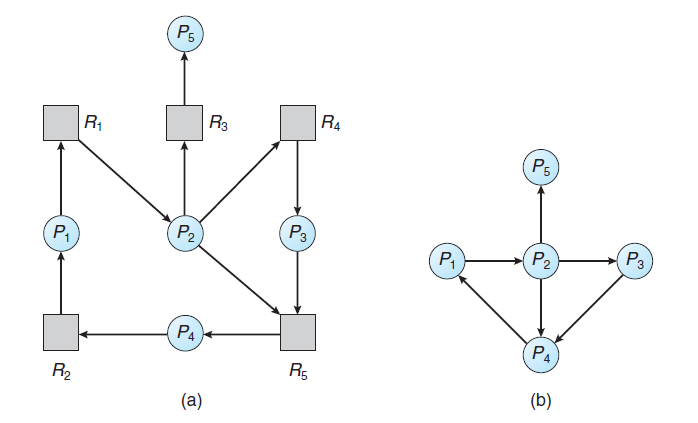
\includegraphics[width=0.75\textwidth]{images/rag-waitfor.png}
	\end{center}

\end{frame}

\begin{frame}
	\frametitle{Cycle Detection}

	Given the wait-for graph, it is trivial for humans to look at this and determine if there is a cycle, but for the computer it takes slightly more work.

	A cycle exists in the wait for graph if and only if a deadlock exists in the system.

	Such cycle detection algorithms tend to have runtime characteristics of $\Theta(n^{2})$ where $n$ is the number of nodes in the graph.

\end{frame}

\begin{frame}
	\frametitle{General Deadlock Detection Algorithm}

	We will use the general deadlock detection algorithm that allows for multiple resources of each type.

	There are $n$ processes numbered $P_{1}$ through $P_{n}$ and $m$ resources.

	Resources are represented by two vectors:\\
	\quad $E$ -- the existing resource vector.\\
	\quad $A$ -- the available resource vector.

	If resource $i$ has two instances total and one is currently assigned to a process, $E_{i}$ is 2 and $A_{i}$ is 1.

\end{frame}

\begin{frame}
	\frametitle{General Deadlock Detection Algorithm}

	We need two matrices to represent the current situation of the system.

	The first is $C$, the current allocation.

	Row $i$ of $C$ shows how many of each resource $P_{i}$ has.

	The second matrix is $R$, the request matrix.

	$C_{ij}$ shows the number of instances of resource $j$ that $P_{i}$ has and $R_{ij}$ shows the number of instances of resource $j$ that $P_{i}$ wants.

\end{frame}

\begin{frame}
	\frametitle{General Deadlock Detection Algorithm}

	\begin{multicols}{2}
		\begin{center}
			\textsf{Resources in Existence}\\
			$[E_{1}, E_{2}, ..., E_{m}]$\vspace{5em}

			\textsf{Current Allocations}
			\[
				\left[ {\begin{array}{cccc}
								C_{11} & C_{12} & ... & C_{1m} \\
								C_{21} & C_{22} & ... & C_{2m} \\
								\vdots & \vdots &     & \vdots \\
								C_{n1} & C_{n2} & ... & C_{nm}
							\end{array} } \right]
			\]
		\end{center}
		\columnbreak

		\begin{center}
			\textsf{Resources Available}\\
			$[A_{1}, A_{2}, ..., A_{m}]$\vspace{3em}

			\textsf{Requests}
			\[
				\left[ {\begin{array}{cccc}
								R_{11} & R_{12} & ... & R_{1m} \\
								R_{21} & R_{22} & ... & R_{2m} \\
								\vdots & \vdots &     & \vdots \\
								R_{n1} & R_{n2} & ... & R_{nm}
							\end{array} } \right]
			\]
		\end{center}

	\end{multicols}

	\begin{center}
		$\sum\limits_{i=1}^n C_{ij} + A_{j} = E_{j}$.
	\end{center}


\end{frame}

\begin{frame}
	\frametitle{Less Than? Says Who?}

	There is one more bit of setup before we are ready to run the algorithm.

	The key idea is comparison of vectors, so let us define for notational convenience, the idea of ``less than'' for two vectors.

	We will say that for two vectors $A$ and $B$ of length $m$,  $A \leq B$ means that $A_{i} \leq B_{i}$ for all $i$ from 1 to $m$.

\end{frame}

\begin{frame}
	\frametitle{Run, Algorithm, Run}

	All processes are unmarked and the vectors and matrices are populated.

	\begin{enumerate}
		\item Search for an unmarked process whose requests can all be satisfied with the available resources in $A$. Mathematically: find a process $P_{i}$ such that row $R_{i} \leq A$.
		\item If a process is found, add the allocated resources of that process to the available vector and mark the process. Mathematically: $A = A + C_{i}$. Go back to step 1.
		\item If no process was found in the search of step 1, the algorithm terminates.
	\end{enumerate}

	At the end, any processes that are not marked are deadlocked.

\end{frame}

\begin{frame}
	\frametitle{General Deadlock Detection Algorithm Analysis}

	This approach is similar to the banker's algorithm.

	Step 1: look for a process that can run to completion; it will be able to do so because the currently available resources equal or exceed its needs.

	That process can finish, and when it does so, its currently-held resources are released and available for another process to acquire.

	Step two reflects this by adding the resources it holds to the available set.

	Then another process is selected.

	At the end, either all processes can finish and there is no deadlock, or there is a set of processes (at least two) that are deadlocked.

	This algorithm has a runtime performance characteristic of $\Theta(m \times n^{2})$.


\end{frame}

\begin{frame}
	\frametitle{Detection of Deadlock Example}
	System initial state (4 resources, 3 processes):

	\begin{multicols}{2}
		\begin{center}
			$E = [4, 2, 3, 1]$
			\[ C =
				\left[ {\begin{array}{cccc}
								0 & 0 & 1 & 0 \\
								2 & 0 & 0 & 1 \\
								0 & 1 & 2 & 0 \\
							\end{array} } \right]
			\]
		\end{center}
		\columnbreak

		\begin{center}
			$A = [2, 1, 0, 0]$
			\[ R =
				\left[ {\begin{array}{cccc}
								2 & 0 & 0 & 1 \\
								1 & 0 & 1 & 0 \\
								2 & 1 & 0 & 0
							\end{array} } \right]
			\]
		\end{center}

	\end{multicols}


\end{frame}


\begin{frame}
\frametitle{I'll Take Your Word For It}

If we have started some operation and it is taking too long, we can assume that a deadlock occurred and decide to take action.

\begin{center}
	
\includegraphics[width=0.5\textwidth]{images/zoidberg.jpg}
\end{center}

This does mean we might declare a deadlock when there really is none.

One way to implement this is via a watchdog timer.

\end{frame}


\begin{frame}
	\frametitle{When to Detect Deadlock}

	The runtime characteristic of the simple deadlock detection algorithm: $\Theta(n^{2})$.

	The runtime characteristic of the general algorithm was shown as $\Theta(m \times n^{2})$.

	($n$ is the number of processes and $m$ is the number of resources in the system)

	This means that the deadlock detection routine is expensive to execute.


\end{frame}

\begin{frame}
	\frametitle{When to Detect Deadlock}

	This prompts a question: how often should the deadlock detection algorithm be run?

	One strategy is to run it every time a resource is requested.

	Optimization: it should run if a resource request cannot be granted.

	Another idea: run it periodically instead.

\end{frame}

\begin{frame}
	\frametitle{When to Detect Deadlock}

	When to run the deadlock detection algorithm depends on how often we expect deadlock to occur, and how severe a problem it is when deadlock occurs.

	If deadlock happens a lot, checking for deadlock often will make sense.

	If the consequences of a deadlock are severe, it makes sense to check frequently to identify the problem as soon as possible.

	Idea: run it when CPU utilization is low...?

\end{frame}


\begin{frame}
	\frametitle{We Can Fix This}

	\begin{center}
		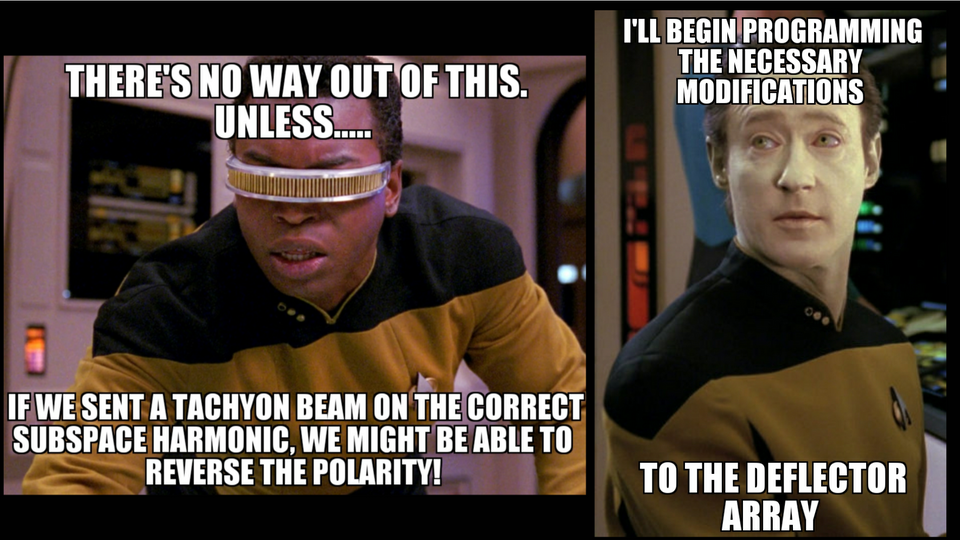
\includegraphics[width=\textwidth]{images/recovery.png}
	\end{center}

\end{frame}


\begin{frame}
	\frametitle{Deadlock Recovery}

	Once a deadlock has been detected, a system can recover from that deadlock by ``breaking'' the deadlock.

	These are called recovery strategies and they are ways the system may automatically deal with the problem.

	It is possible to have a manual form of deadlock recovery, where an operator is notified and that person is responsible for sorting out the problem.

	The manual method needs no further discussion.


\end{frame}

\begin{frame}
	\frametitle{Recovery Strategies}

	There are several strategies that we could apply.

	They can result in data loss, delays in completion, other problems...

	Ideally we would like to break the deadlock with as little disruption as possible, so the strategies that rely on selection of victims should choose carefully.

	These strategies are not mutually exclusive.

\end{frame}


\begin{frame}
	\frametitle{Here's One Idea}

	\begin{center}
		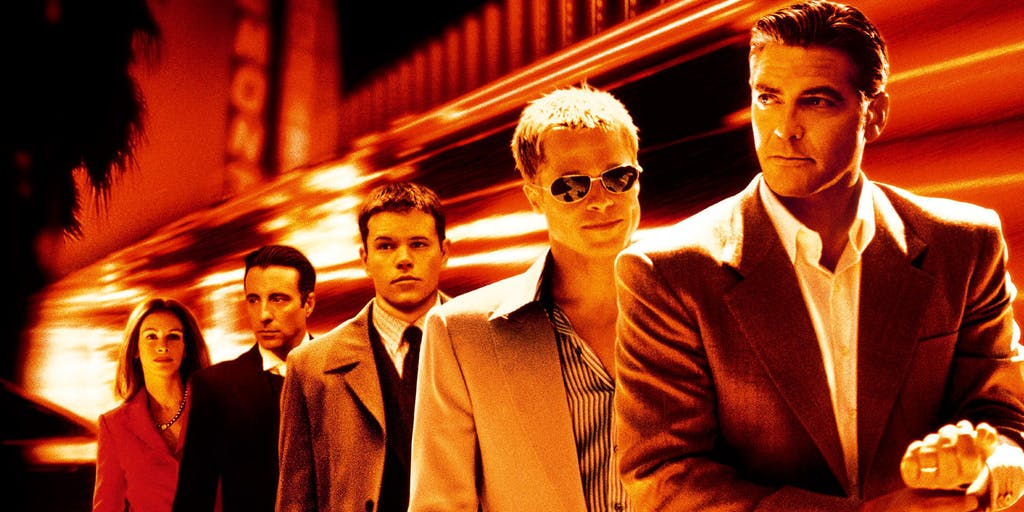
\includegraphics[width=\textwidth]{images/oceans-eleven.jpeg}
	\end{center}

\end{frame}


\begin{frame}
	\frametitle{Robbery}

	The strategy of ``robbery'' is just a humorous way of saying preemption.

	This is virtually identical to the discussion of deadlock prevention.\\
	\quad But it happens  only when deadlock is detected.

	The operating system needs to choose a victim to rob...

	The resource should be an appropriate type to be preempted!


\end{frame}

\begin{frame}
	\frametitle{Robbery}


	Suppose $P_{1}$ has a resource $R_{1}$ and needs $R_{2}$, while $P_{2}$ has $R_{2}$ and needs $R_{1}$.

	The OS may block $P_{2}$ and take away $R_{2}$ from $P_{2}$ and allow $P_{1}$ to have it.

	After that resource becomes available again, it is returned to $P_{2}$.


\end{frame}

\begin{frame}
	\frametitle{Mass Murder}

	\begin{center}
		
\includegraphics[width=0.65\textwidth]{images/killemall.jpg}
	\end{center}

\end{frame}

\begin{frame}
	\frametitle{Mass Murder}

	Terminate (kill) all the processes involved in the deadlock.

	This solution is surprisingly common.

	It is one way to be certain that the deadlock cycle is broken.

	The resources that these processes were holding will become available.

	There is no need to determine a victim: kill 'em all and let root sort them out.

\end{frame}

\begin{frame}
	\frametitle{Mass Murder}

	This solution, while easy to implement, may not solve the problem.

	The circumstances that caused the deadlock may occur again.

	If the deadlock were an unlikely situation caused by ``unlucky'' timing then it will probably not recur, or at least, will not recur for some time.

	If $P_{1}$ and $P_{2}$ are deadlocked, however, is it really necessary to kill both?

	If we killed only one, the other could proceed...

\end{frame}


\begin{frame}
	\frametitle{Hello, Clarice...}

	\begin{center}
		
\includegraphics[width=\textwidth]{images/mikkelsen.jpg}
	\end{center}

\end{frame}


\begin{frame}
	\frametitle{Murder}

	Perhaps instead of killing all processes involved in a deadlock, the operating system chooses to kill processes selectively.

	Like preemption, selecting which process is the victim is important.

	When the victim is killed, its resources are added to the available set and this will hopefully allow other processes to proceed.

\end{frame}

\begin{frame}
	\frametitle{Murder}
	Run the deadlock detection algorithm again to determine if deadlock still exists.

	If so, this strategy needs to be repeated.

	Repeat until the logjam is broken.

	Presumably kills fewer processes than the ``mass murder'' strategy.

\end{frame}


\begin{frame}
	\frametitle{Next Idea: Back we Go...}

	\begin{center}
		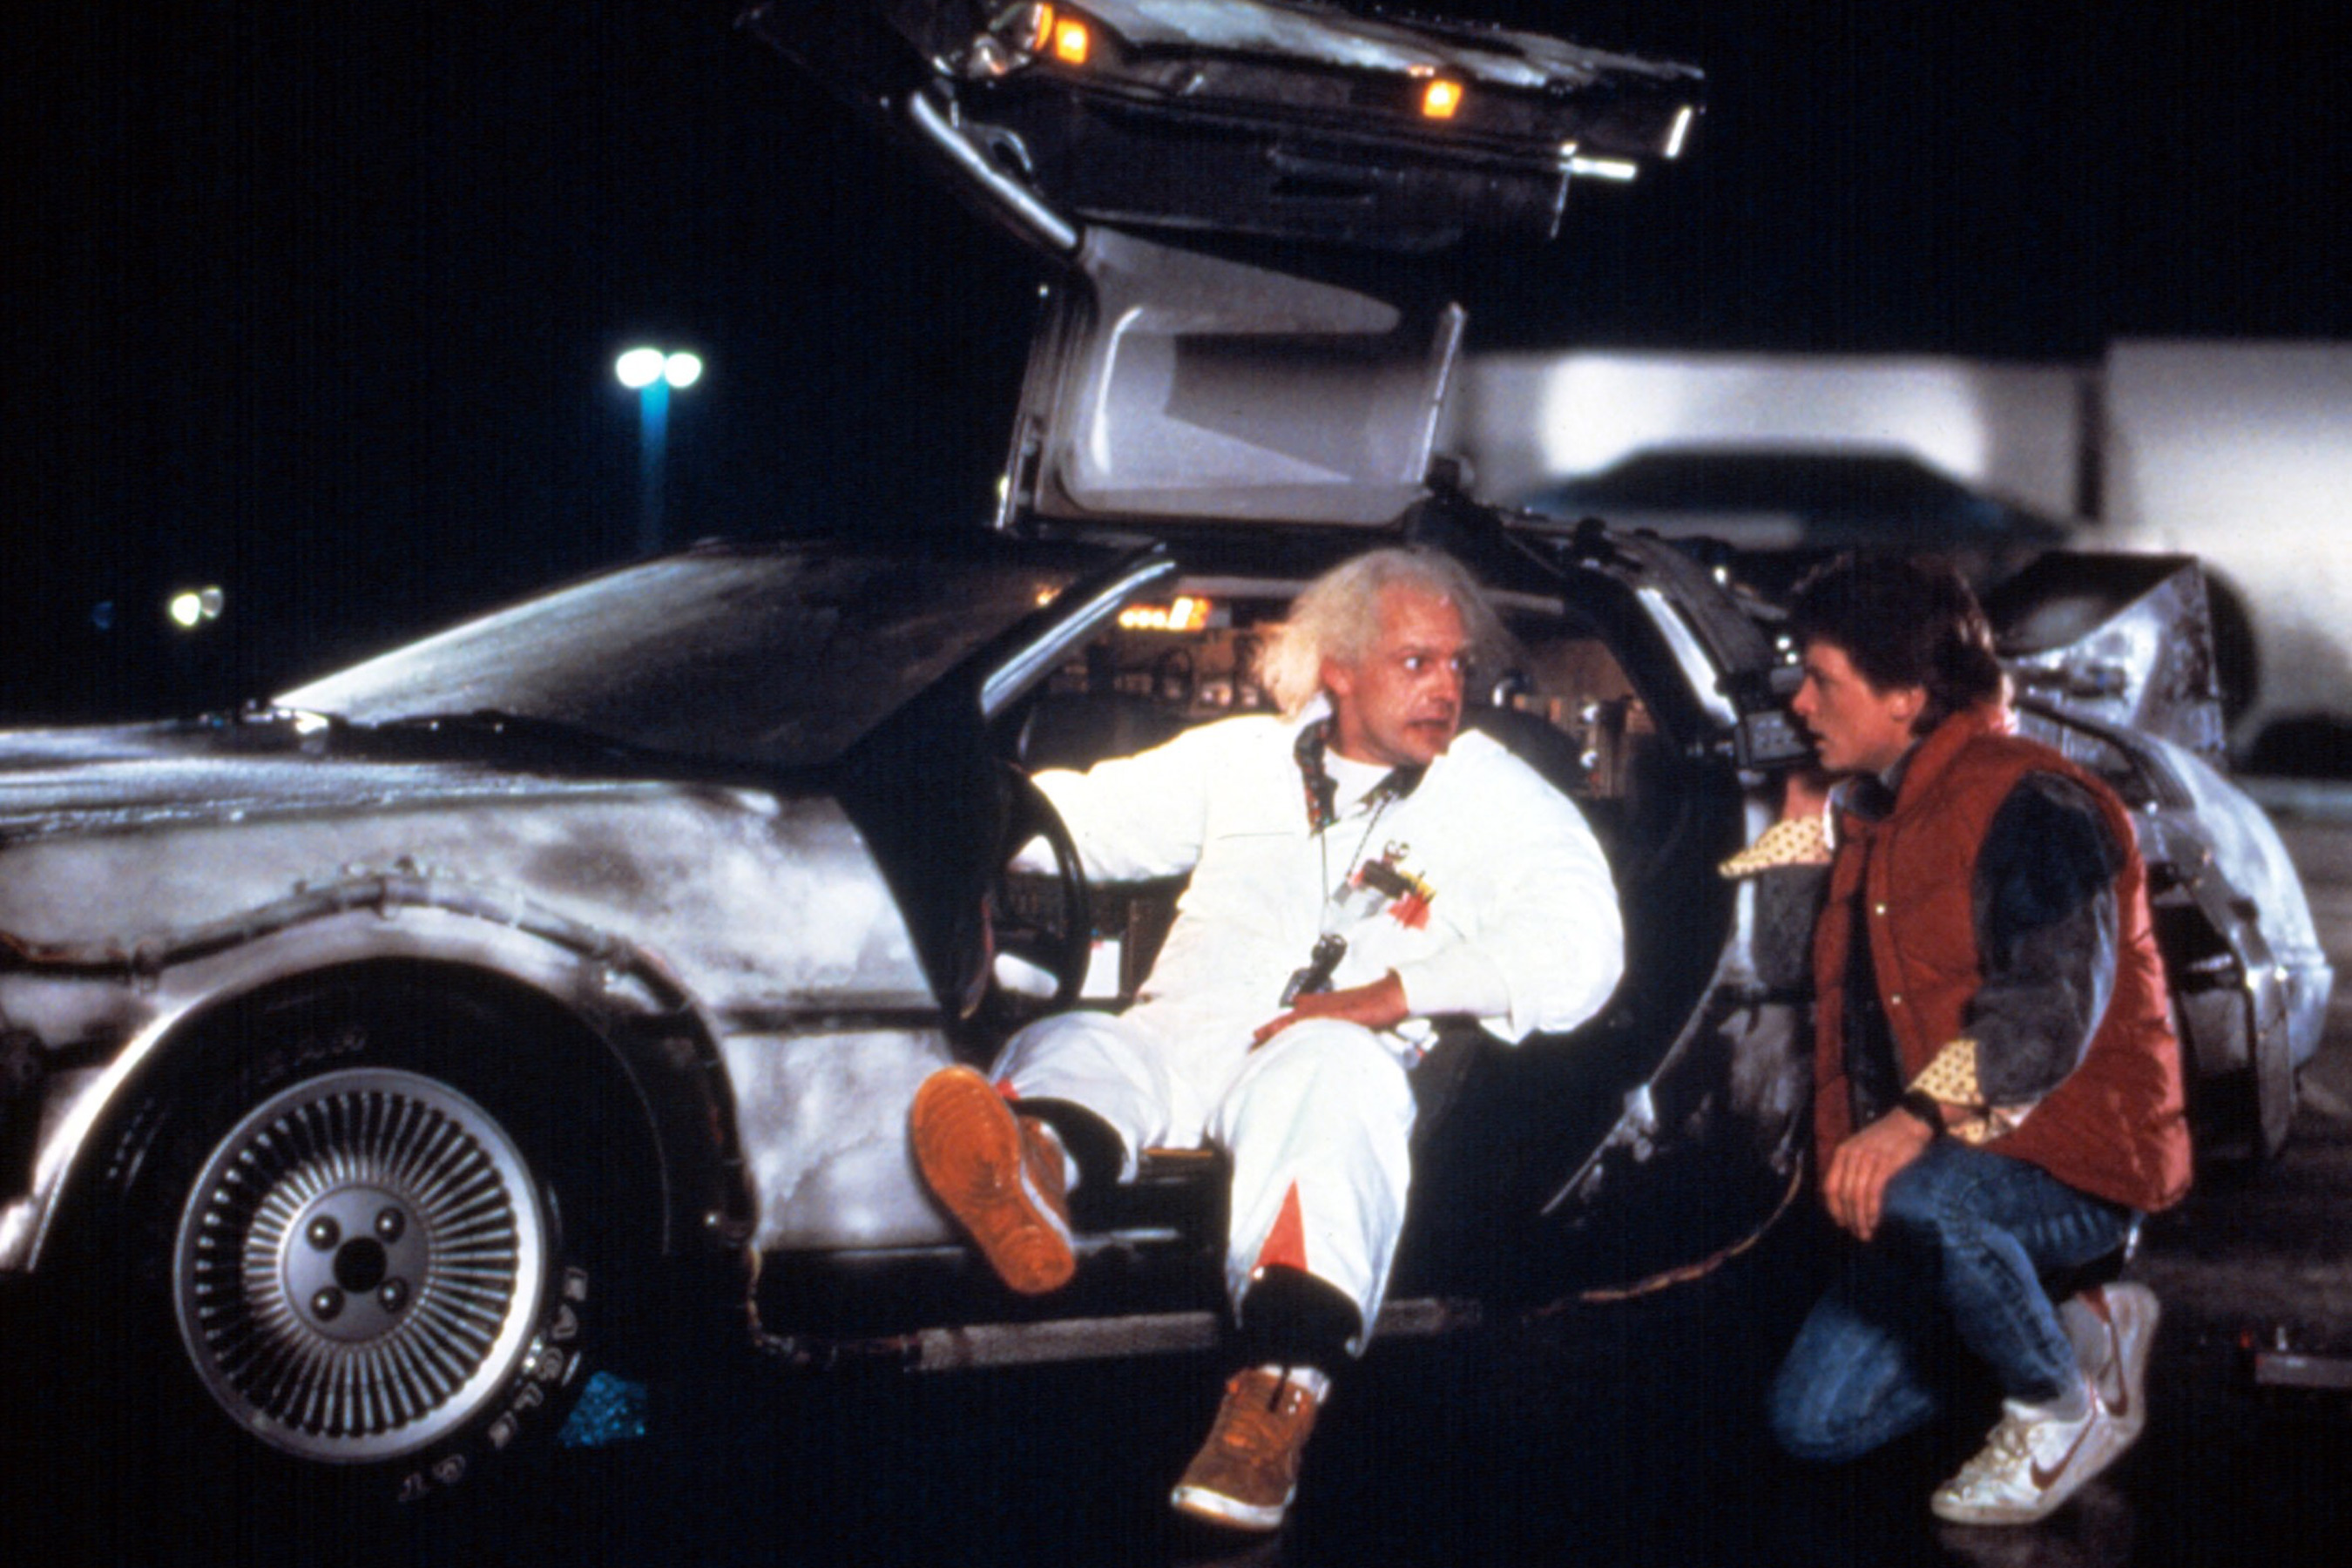
\includegraphics[width=\textwidth]{images/bttf.jpg}
	\end{center}

\end{frame}


\begin{frame}
	\frametitle{Time Travel}

	\alert{Rollback}: returning the state of a process to a saved state from an earlier time.

	There must be a saved state that was created in advance of a problem. \\
	\quad Otherwise there is no state to roll back to!

	The saved state is called a \alert{checkpoint} and the act of creating and saving a checkpoint is called \alert{checkpointing}.

	Checkpoints may be created periodically or before beginning a particular operation that requires a lot of resources.

\end{frame}

\begin{frame}
	\frametitle{Time Travel}

	A checkpoint contains the memory image, including the call stack, and resource state of a process.

	It is written to disk and will usually persist as long as the process executes.

	You might already be somewhat familiar with the concept of rollbacks if you have used version control software like Subversion (\texttt{svn}) or Git (\texttt{git}).

	Rollbacks are also common in databases.

\end{frame}

\begin{frame}
	\frametitle{Time Travel}

	Unfortunately, rollback does not always succeed.

	Sometimes moving the process back to an earlier state just moves it a few steps back on the same road that leads to the deadlock.

	Rollback may be attempted a few times before trying another strategy.

\end{frame}


\begin{frame}
	\frametitle{Armageddon}

	\begin{center}
		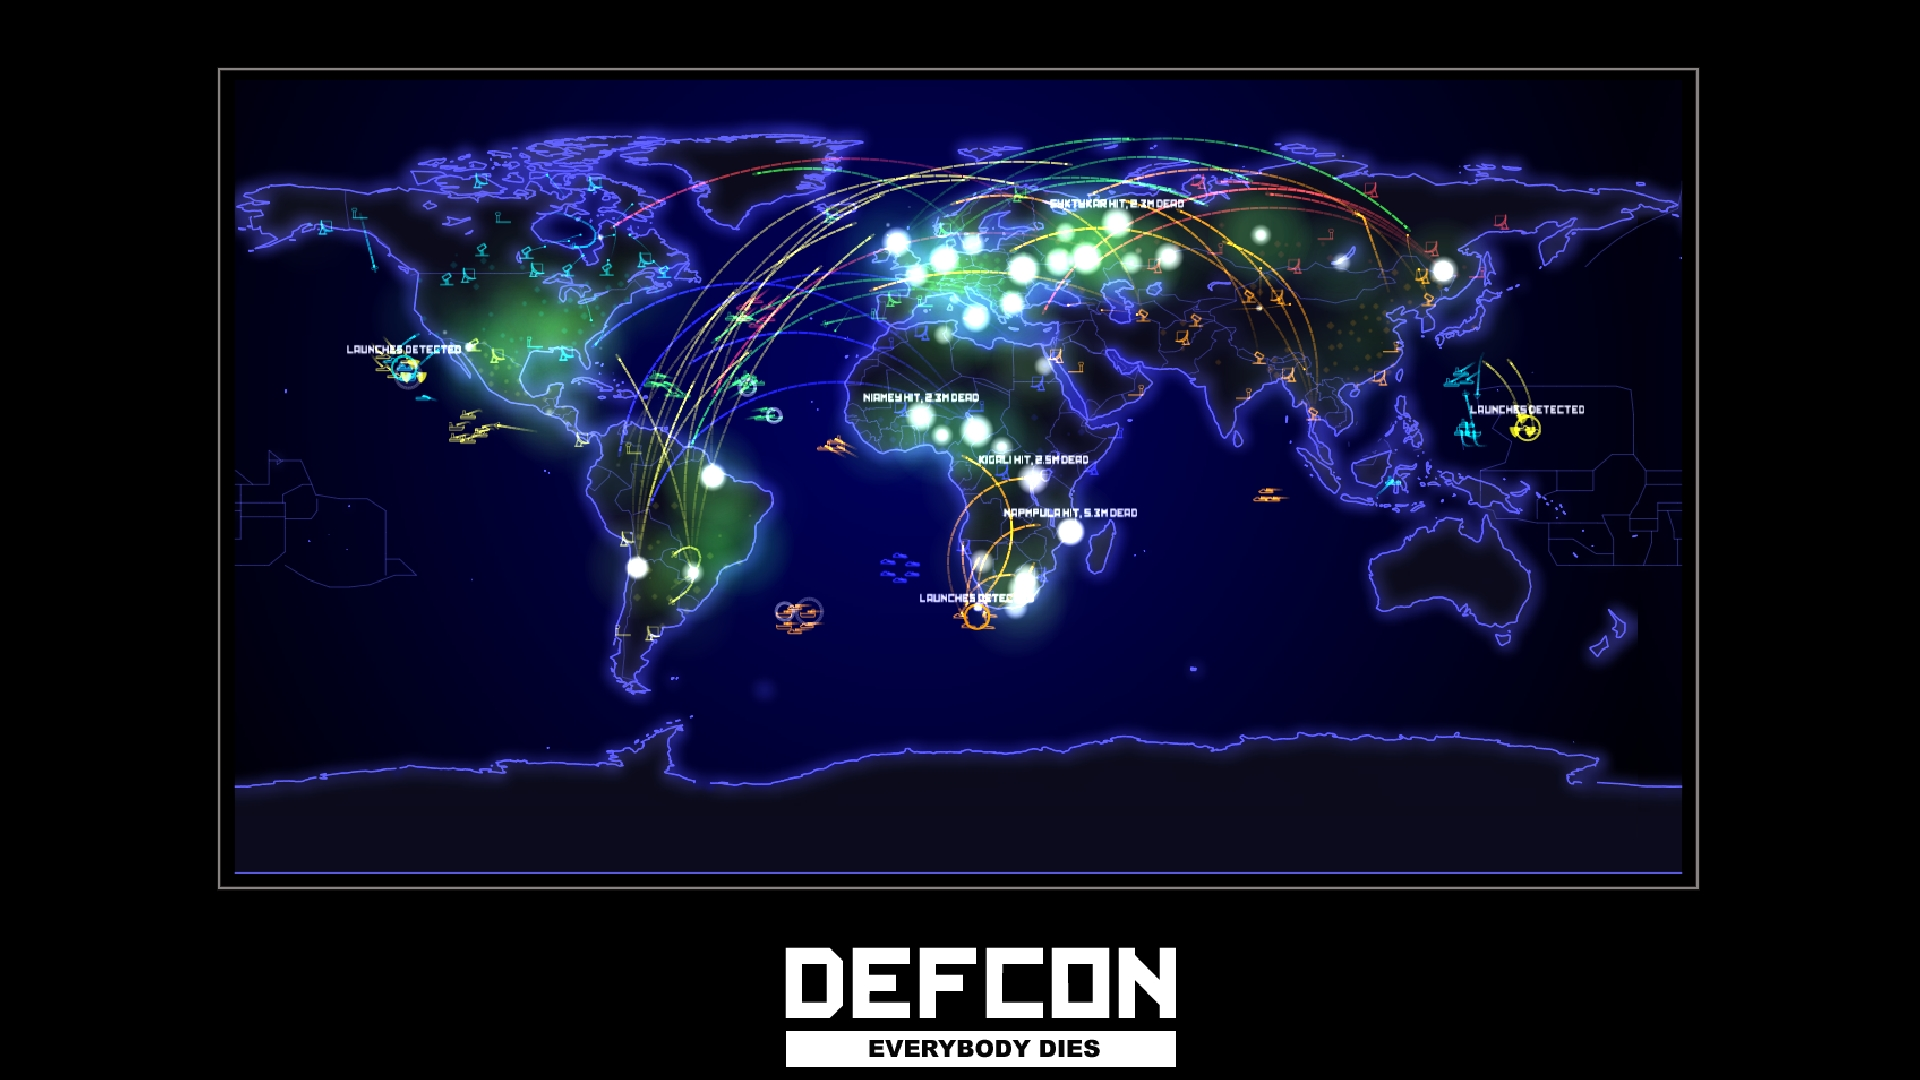
\includegraphics[width=\textwidth]{images/defcon.jpg}
	\end{center}

\end{frame}


\begin{frame}
	\frametitle{Armageddon}

	Armageddon - the end of the world.

	If a deadlock has occurred, sometimes the best thing to do is reboot the system.

	This has a side effect of killing all processes, whether they are stuck or not, but is sometimes the best way to make sure that the system is in a valid state.

	NASA's Spirit rover relies on this strategy if it detects a deadlock.

	Like killing all affected processes, it is easy to implement, but is most disruptive.

\end{frame}

\begin{frame}
	\frametitle{Victim Selection}

	If we have to choose a victim process for one of the strategies, e.g., termination, then we need a strategy for which process to choose.

	We could choose randomly: kill a process and hope that that was enough.

	Sometimes this will work, because it breaks the deadlock and the other processes can all proceed.

	In general, however, making an informed decision is better.

\end{frame}

\begin{frame}
	\frametitle{(Don't) Shoot Innocent Bystanders}

	It is not necessary to choose one of the processes involved in the deadlock.

	If $P_{1}$ and $P_{2}$ are deadlocked, $P_{3}$  may have an instance of a resource $P_{1}$ needs.

	Killing $P_{3}$ will allow both $P_{1}$ and $P_{2}$ to proceed.

\end{frame}

\begin{frame}
	\frametitle{Victim Selection: An Optimization Problem}

	Define a cost function for choosing each process, evaluate it, choose the lowest.

	Some factors to consider:

	\begin{enumerate}
		\item The priority of the process.
		\item How long the process has been executing.
		\item How long is remaining in execution, if known.
		\item What resources the process has (number and type).
		\item Future resource requests, if known.
		\item Whether the process is user-interactive or in the background.
		\item How many times, if any, the process has been selected as a victim.
	\end{enumerate}

\end{frame}

\begin{frame}
	\frametitle{Geri and the Atrics}

	Selection routines tend to favour older processes rather than younger ones.

	This is not because older processes vote in higher numbers, but because it tends to be more expensive to restart an older process.

	A process that has been running for a long time, if it is restarted, has to do a lot more work to get to the point where it was terminated than a younger process.

\end{frame}

\begin{frame}
	\frametitle{Geri and the Atrics}

	If the oldest process were constantly the one selected, that process itself might never get to run to completion (starvation).

	If the killing process is very aggressive then no tasks run to completion because each process, shortly after becoming the oldest, is killed.


	Therefore, young processes tend to be the ones selected.

\end{frame}

\begin{frame}
	\frametitle{Keeping Track}

	The final element in the list, keeping track of how many times a process has been victimized, is also there to prevent starvation.

	The selection process very likely produces the same or similar results each time it is run, so it may happen that the same process is selected over and over again.

	It may be advisable to take the number of rollbacks or terminations into account so that no process in particular is starved.

\end{frame}

\begin{frame}
	\frametitle{Miscarriages of Justice}

	The deadlock detection algorithm we have chosen tends to be conservative.\\
	\quad It will err on the side of saying that there is a deadlock.

	The worst case is assumed: that processes take resources and keep them until the end of their execution.

	We might detect a deadlock when there is none.

	We may also, then, kill an innocent process in a system that is not actually deadlocked. Oops!

\end{frame}

\begin{frame}
	\frametitle{It's Okay to Make Mistakes}

	It turns out that our deadlock detection algorithms do not have to be perfect if we have chosen an appropriate recovery strategy.

	If killing the process and restarting it does not have unexpected side effects, then being selected does not have an impact on the correctness of the program.

	... Only on how long it takes to execute.

	For example, the victim process is a compiler.

	If killed and started again, it takes slightly longer for the compile to finish, but there is no impact on the correctness of the binary.

\end{frame}


\begin{frame}
\frametitle{Lifelock}

\begin{center}
	
\includegraphics[width=0.7\textwidth]{images/lifelock.jpg}
\end{center}

No, wait, that's not quite correct.

\end{frame}


\begin{frame}
\frametitle{Lifelock}

\begin{center}
	
\includegraphics[width=0.5\textwidth]{images/zoidberg2.jpg}
\end{center}

Better.

But we actually wanted to talk about Livelock.

\end{frame}


\begin{frame}
\frametitle{Livelock}

	Ideally, our recovery strategy is effective: some threads continue.
	
	Unfortunately, sometimes we just end up at the same impasse again.
	
	Deadlock recovery strategies are not the only way to end up in livelock.
	
	Imagine the dining philosophers, perfectly synchronized.

\end{frame}


\begin{frame}
\frametitle{Full of Sound and Fury, Signifying Nothing}

	In real life, it is unlikely that $n$ threads executing on a general purpose operating system would achieve this sort of perfect lock-step.
	
	Even so, livelock can occur in long-running tasks.

	Problem: this is harder to detect than deadlock. Why?
\end{frame}


\begin{frame}
\frametitle{Full of Sound and Fury, Signifying Nothing}

	In deadlock, threads are known to be blocked and analysis tools (e.g., a debugger) can tell you at what statement those threads are blocked.
	
	With livelock, it seems like the threads are running and working, but somehow no work is getting done. 

	For this reason, a well-designed recovery strategies may have some sort of limit on the number of retries...

\end{frame}



\end{document}

